\documentclass[preprint,12pt,aps,pra,showkeys,amsmath,amssymb,superscriptaddress,floatfix]{revtex4-2}
\usepackage[T1]{fontenc}
\usepackage[utf8]{inputenc}
\usepackage{amsmath,amssymb,amsthm,mathtools,mathrsfs}
\usepackage{microtype,booktabs,enumitem}
\usepackage{xcolor,tikz,etoolbox}
\usepackage[skins,breakable]{tcolorbox}
\usepackage{needspace}
% Keep diagram geometry independent of REVTeX preprint body spacing.
\AtBeginEnvironment{tikzpicture}{\linespread{1}\selectfont}
\usetikzlibrary{arrows.meta,positioning,calc,fit,decorations.pathreplacing}
\usepackage{graphicx}
\usepackage{hyperref}

\definecolor{MMBlue}{RGB}{0,82,155}
\definecolor{MMOrange}{RGB}{200,80,0}
\tikzset{
 mmnode/.style={draw=MMBlue,rounded corners=2pt,fill=MMBlue!4,align=left,execute at begin node={\raggedright},text width=5cm,font=\fontsize{10}{12}\selectfont,inner sep=6pt},
 mmimport/.style={mmnode,draw=black!65,fill=black!4},
 mmcandidate/.style={mmnode,draw=MMOrange,dashed,fill=MMOrange!5},
 mmrejected/.style={mmnode,draw=black,densely dotted,fill=black!8},
 mmproof/.style={->,thick,MMBlue},
 mmflow/.style={->,semithick,black!70},
 mmrepair/.style={->,dashed,thick,MMOrange},
 mmcandidatearrow/.style={->,dashed,semithick,MMOrange},
 mmnote/.style={font=\scriptsize,fill=white,inner sep=2pt,align=center}}

\usepackage[section]{placeins}
\setlength{\emergencystretch}{3em}
\setlist{itemsep=3pt,topsep=4pt}
\newtheorem{theorem}{Theorem}[section]
\newtheorem{proposition}[theorem]{Proposition}
\newtheorem{lemma}[theorem]{Lemma}
\newtheorem{corollary}[theorem]{Corollary}
\theoremstyle{definition}
\newtheorem{definition}[theorem]{Definition}
\newtheorem{example}[theorem]{Example}
\theoremstyle{remark}
\newtheorem{remark}[theorem]{Remark}
% Avoid isolated statement headings and single-line paragraph fragments.
\BeforeBeginEnvironment{theorem}{\Needspace{6\baselineskip}}
\BeforeBeginEnvironment{definition}{\Needspace{5\baselineskip}}
\BeforeBeginEnvironment{proposition}{\Needspace{5\baselineskip}}
\BeforeBeginEnvironment{lemma}{\Needspace{5\baselineskip}}
\BeforeBeginEnvironment{corollary}{\Needspace{5\baselineskip}}
\clubpenalty=5000
\widowpenalty=5000
\newcommand{\R}{\mathbb R}\newcommand{\Z}{\mathbb Z}\newcommand{\N}{\mathbb N}
\newcommand{\Pa}{\operatorname{Pa}}\newcommand{\Desc}{\operatorname{Desc}}
\newcommand{\cl}{\operatorname{cl}}\newcommand{\cost}{\operatorname{cost}}
\newcommand{\status}{\operatorname{status}}
% Faculty cards: a visual rail groups the five faculties within one agent.
% The rail has no arrowhead and does not represent a proof dependency.
\newcommand{\mmfacultybadge}[1]{%
 \node[circle,draw=MMBlue,line width=1pt,fill=white,
 minimum size=7mm,inner sep=0pt,font=\sffamily\small\bfseries,text=MMBlue]
 at ([xshift=15pt,yshift=-15pt]frame.north west) {#1};}
\newcommand{\mmfacultyrail}{%
 \draw[MMBlue!80,line width=1pt]
 ([xshift=15pt,yshift=2pt]frame.north west)--
 ([xshift=15pt,yshift=-2pt]frame.south west);}
\newtcolorbox{mmfacultybox}[2]{enhanced,breakable,
 colback=MMBlue!4,colframe=MMBlue!4,boxrule=0pt,arc=3pt,
 left=39pt,right=9pt,top=4pt,bottom=4pt,
 before skip=2pt,after skip=2pt,
 fontupper=\small\linespread{1.1}\selectfont,
 overlay unbroken={\mmfacultyrail\mmfacultybadge{#1}},
 overlay first={\mmfacultyrail\mmfacultybadge{#1}},
 overlay middle={\mmfacultyrail},overlay last={\mmfacultyrail}}
\newcommand{\mmfaculty}[3]{%
 \begin{mmfacultybox}{#1}{#2}
 {\sffamily\bfseries\color{MMBlue}#2}\par\smallskip #3
 \end{mmfacultybox}}
\newcommand{\agent}[9]{%
 \Needspace{8\baselineskip}
 \subsubsection{#1}
 \noindent\textbf{Object.} #2\par
 \noindent\textbf{Role.} #3\par\smallskip
 \mmfaculty{E}{Ego}{#4}
 \mmfaculty{M}{Memory}{#5}
 \mmfaculty{I}{Intellect}{#6}
 \mmfaculty{S}{Sense}{#7}
 \mmfaculty{A}{Action}{#8}
 \smallskip\noindent #9\par}

\usepackage{longtable,array,calc}
\providecommand{\tightlist}{\setlength{\itemsep}{2pt}\setlength{\parskip}{0pt}}
\makeatletter
\def\frontmatter@abstract@produce{\par\addvspace{\frontmatter@preabstractspace}%
\begingroup\prep@absbox\unvbox\absbox\post@absbox\endgroup
\addvspace{\frontmatter@postabstractspace}}
\makeatother
\newcommand{\field}[2]{\par\smallskip\noindent\textbf{#1.} #2\par}
\setlength{\emergencystretch}{5em}
\AtBeginEnvironment{verbatim}{\small\linespread{1.0}\selectfont}


\hypersetup{colorlinks=true,linkcolor=MMBlue,urlcolor=MMBlue,pdfauthor={Dibakar Sigdel}}

\begin{document}

\title{Cantor--Schröder--Bernstein Theorem\\[4pt]\large An End-to-End Meta-Math Walkthrough}

\author{Dibakar Sigdel}

\affiliation{Mindverse Computing LLC, Lynnwood, WA 98087, USA}

\date{October 2026}

\begin{abstract}

Start chains at the part of \(A\) not hit by \(g\). Follow \(g\circ f\)
forward from those starts; use \(f\) on that chain region and reverse
\(g\) everywhere else. The report presents the target theorem, declared
imports, a dependency graph, five-faculty node contracts, a continuous
proof, a worked example, and a hypothesis-repair audit. It is an
authored mathematical exposition, not a deployed-agent transcript or a
formal proof-assistant certificate.

\end{abstract}\maketitle\linespread{1.12}\selectfont

\noindent\textbf{LF-02 / Mathematical Logic and Set Theory / Report v1}

\section{Target and import contract}

\begin{theorem}

If injections \(f:A\to B\) and \(g:B\to A\) exist, prove there is a
bijection \(h:A\to B\). The construction works for arbitrary sets and
does not need a choice of preimages beyond the unique preimages already
supplied by an injection.

\end{theorem}

\subsection{Foundations and permitted imports}

Use ordinary set operations, recursion over \(\mathbb N\), and
injectivity. The notation \(g^{-1}(a)\) below refers to the unique
preimage of \(a\in g(B)\); it is not defined on all of \(A\). No
cardinal arithmetic or axiom of choice is needed for the proof.

\clearpage\section{Node interaction workflow}

\begin{center}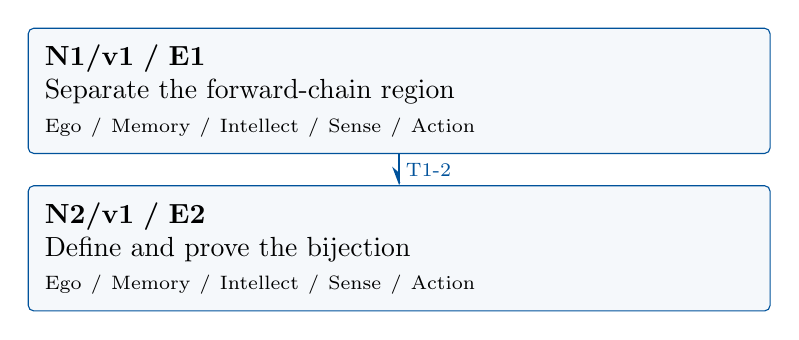
\begin{tikzpicture}[>=Stealth,x=1cm,y=1cm]

\node[mmnode,text width=9cm,minimum height=1.25cm] (N1) at (0,0.0) {\textbf{N1/v1 / E1}\\Separate the forward-chain region\\{\scriptsize Ego / Memory / Intellect / Sense / Action}};

\node[mmnode,text width=9cm,minimum height=1.25cm] (N2) at (0,-2.0) {\textbf{N2/v1 / E2}\\Define and prove the bijection\\{\scriptsize Ego / Memory / Intellect / Sense / Action}};

\draw[mmproof] (N1.south) -- node[mmnote,right] {T1-2} (N2.north);

\end{tikzpicture}\end{center}

Each box is one mathematical agent containing all five faculties. Blue
arrows carry the versioned exports listed below. The layout gives a
reading order; only drawn arrows assert dependencies. Diagnostic repair
is separate from the proof DAG.

\subsection{Versioned evidence-transfer ledger}

\begingroup\small\linespread{1.05}\selectfont

\Needspace{5\baselineskip}\field{T1-2: N1/E1/v1 to N2}{\(C\cap g(B)=g(f(C))\) and \(A\setminus C\subset g(B)\).}

\field{Receiving activity}{N2.1}

\field{Compatibility}{E1/v1 and \(h(a)=f(a)\) for \(a\in C\), \(h(a)=g^{-1}(a)\) for
\(a\notin C\). Check: Injectivity on each branch alone does not rule out
collisions across branches.}

\endgroup

\clearpage\section{Agent roles and five-faculty activities}\begingroup\small\linespread{1.05}\selectfont\setlist{itemsep=1pt,topsep=2pt}

\subsection{N1/v1: Separate the forward-chain region}

\field{Object and role}{Identify exactly which elements of the chain region lie in the image of
\(g\). \textbf{Local obligation:} \(C\cap g(B)=g(f(C))\) and
\(A\setminus C\subset g(B)\).}

\field{Inputs}{\(A_0=A\setminus g(B)\), \(A_{n+1}=g(f(A_n))\), and
\(C=\bigcup_{n\ge0}A_n\).}

\mmfaculty{E}{Ego}{Publish E1/v1 only after establishing this obligation:
\(C\cap g(B)=g(f(C))\) and \(A\setminus C\subset g(B)\).}

\mmfaculty{M}{Memory}{\(A_0=A\setminus g(B)\), \(A_{n+1}=g(f(A_n))\), and
\(C=\bigcup_{n\ge0}A_n\). Retain the stated assumptions and import
versions.}

\mmfaculty{I}{Intellect}{Identify exactly which elements of the chain region lie in the image of
\(g\).}

\mmfaculty{S}{Sense}{Every point outside \(C\) is in \(g(B)\) because \(A_0\subset C\).}

\mmfaculty{A}{Action}{Carry out activities N1.1--N1.2 below, retaining each calculation and
construction as evidence.}

\smallskip\noindent\textbf{Numbered mathematical activities}

\begin{enumerate}[label=N1.\arabic*,leftmargin=3.4em]

\item Every \(A_n\) with \(n\ge1\) lies in \(g(B)\), whereas \(A_0\) is
disjoint from \(g(B)\). Hence \(C\cap g(B)=\bigcup_{n\ge1}A_n\).

\item Images commute with unions, so
\(g(f(C))=\bigcup_{n\ge0}g(f(A_n))=\bigcup_{n\ge1}A_n\). This proves the
equality. Also if \(a\notin C\), it cannot belong to
\(A_0=A\setminus g(B)\), so it lies in \(g(B)\).

\end{enumerate}

\field{Export E1/v1}{\(C\cap g(B)=g(f(C))\) and \(A\setminus C\subset g(B)\).}

\field{Acceptance gate}{Every point outside \(C\) is in \(g(B)\) because \(A_0\subset C\).}

\field{Targeted repair}{If \(g^{-1}\) is used outside its image, first prove the complement
inclusion; it is what makes the second branch legitimate. Withhold this
export and recheck its descendants after a versioned correction.}

\clearpage

\subsection{N2/v1: Define and prove the bijection}

\field{Object and role}{Prove the two branch images are disjoint and together exhaust \(B\).
\textbf{Local obligation:} The piecewise-defined \(h:A\to B\) is a
bijection.}

\field{Inputs}{E1/v1 and \(h(a)=f(a)\) for \(a\in C\), \(h(a)=g^{-1}(a)\) for
\(a\notin C\). Incoming proof exports: E1/v1 at N2.1.}

\mmfaculty{E}{Ego}{Publish E2/v1 only after establishing this obligation: The
piecewise-defined \(h:A\to B\) is a bijection.}

\mmfaculty{M}{Memory}{E1/v1 and \(h(a)=f(a)\) for \(a\in C\), \(h(a)=g^{-1}(a)\) for
\(a\notin C\). Incoming proof exports: E1/v1 at N2.1. Retain the stated
assumptions and import versions.}

\mmfaculty{I}{Intellect}{Prove the two branch images are disjoint and together exhaust \(B\).}

\mmfaculty{S}{Sense}{Injectivity on each branch alone does not rule out collisions across
branches.}

\mmfaculty{A}{Action}{Carry out activities N2.1--N2.2 below, retaining each calculation and
construction as evidence.}

\smallskip\noindent\textbf{Numbered mathematical activities}

\begin{enumerate}[label=N2.\arabic*,leftmargin=3.4em]

\item E1 makes \(h\) well defined. Each branch is injective. If \(a\in C\) and
\(a'\notin C\) had \(f(a)=g^{-1}(a')\), then
\(a'=g(f(a))\in g(f(C))\subset C\), a contradiction. Thus cross-branch
collisions are impossible.

\item For \(b\in B\), if \(b\in f(C)\) it is hit by the first branch.
Otherwise \(g(b)\notin C\): if it were in \(C\cap g(B)=g(f(C))\),
injectivity of \(g\) would force \(b\in f(C)\). Thus
\(g(b)\in A\setminus C\), and the second branch maps it to \(b\). This
proves surjectivity and hence bijectivity.

\end{enumerate}

\field{Export E2/v1}{The piecewise-defined \(h:A\to B\) is a bijection.}

\field{Acceptance gate}{Injectivity on each branch alone does not rule out collisions across
branches.}

\field{Targeted repair}{If surjectivity is asserted from the two original injections, explicitly
split \(b\) according to membership in \(f(C)\) and use E1 to identify
its branch. Withhold this export and recheck its descendants after a
versioned correction.}

\endgroup\clearpage\section{Continuous mathematical proof}\label{sec:proof}

\subsection{N1 --- Separate the forward-chain
region}\label{n1-separate-the-forward-chain-region}

\begin{enumerate}
\def\labelenumi{\arabic{enumi}.}
\item
  \textbf{N1.1.} Every \(A_n\) with \(n\ge1\) lies in \(g(B)\), whereas
  \(A_0\) is disjoint from \(g(B)\). Hence
  \(C\cap g(B)=\bigcup_{n\ge1}A_n\).
\item
  \textbf{N1.2.} Images commute with unions, so
  \(g(f(C))=\bigcup_{n\ge0}g(f(A_n))=\bigcup_{n\ge1}A_n\). This proves
  the equality. Also if \(a\notin C\), it cannot belong to
  \(A_0=A\setminus g(B)\), so it lies in \(g(B)\).
\end{enumerate}

\subsection{N2 --- Define and prove the
bijection}\label{n2-define-and-prove-the-bijection}

\begin{enumerate}
\def\labelenumi{\arabic{enumi}.}
\item
  \textbf{N2.1.} E1 makes \(h\) well defined. Each branch is injective.
  If \(a\in C\) and \(a'\notin C\) had \(f(a)=g^{-1}(a')\), then
  \(a'=g(f(a))\in g(f(C))\subset C\), a contradiction. Thus cross-branch
  collisions are impossible.
\item
  \textbf{N2.2.} For \(b\in B\), if \(b\in f(C)\) it is hit by the first
  branch. Otherwise \(g(b)\notin C\): if it were in
  \(C\cap g(B)=g(f(C))\), injectivity of \(g\) would force
  \(b\in f(C)\). Thus \(g(b)\in A\setminus C\), and the second branch
  maps it to \(b\). This proves surjectivity and hence bijectivity.
\end{enumerate}

\hfill$\square$

\section{Worked orchestration}

Take \(A=B=\mathbb N_0\), \(f(n)=n+1\), and \(g(n)=n+1\). Then
\(A_0=\{0\}\), \(A_n=\{2n\}\), and \(C\) is the set of even numbers. The
constructed bijection sends even \(n\) to \(n+1\) and odd \(n\) to
\(n-1\), swapping every adjacent pair. This verifies both branches and
their disjoint images.

\subsection{Boundary and hypothesis audit}

A piecewise choice of two injective rules can fail globally: on
\(\{0,1\}\), assign \(0\mapsto0\) on the first singleton branch and
\(1\mapsto0\) on the second. Each restricted map is injective, but the
combined map is not. The cross-branch argument above is therefore an
essential proof obligation.

\section{Illustrative failure and repair}

The following is an authored diagnostic scenario. Changed assumptions
define a new contract; they do not retroactively prove the original
statement.

\subsection{Rejected argument, diagnosis, and correction}
\textbf{Rejected N2 proof:} both pieces are injective, so \(h\) is
injective. \textbf{Sense:} the two-singleton example isolates the
missing cross-case. \textbf{Repair:} assume a cross collision and apply
\(g\) to derive \(a'\in g(f(C))\subset C\), contradicting its branch
membership. This fills the gap with no change of assumptions; recheck
bijectivity after surjectivity is also established.

\subsection{Publication and reuse}
The corrected export retains its explicit assumptions. A hypothetical
revision receives a new version, and each consuming activity is
rechecked; this scenario is not a recorded runtime event. \textbf{Next
direction:} Use explicit injections to compare infinite structures while
retaining this construction as the justification for turning two
inequalities into a bijection.

\par\medskip\begingroup\small\linespread{1.0}\selectfont\noindent\textbf{Provenance.} This authored proof is complete relative to its declared imports. Reuse
each export with its assumptions, proof, and version. The original
Markdown remains available for comparison.
\par\endgroup

\par\smallskip\begingroup\small\linespread{1.0}\selectfont\noindent\textbf{Further reading.} \href{https://math.berkeley.edu/~marks/notes/set_theory_notes_4.pdf}{Andrew
Marks, Set Theory notes} for sets and ultraproducts;
\href{https://math.berkeley.edu/~antonio/math125A/mathlogicP1.pdf}{Berkeley,
Mathematical Logic for Mathematicians, Part I} for first-order
semantics;
\href{https://math.berkeley.edu/~marks/notes/computability_notes_v1.pdf}{Andrew
Marks, Computability Theory notes} for effective procedures and
undecidability. The proofs below specify their own set-theoretic and
semantic assumptions.\par\endgroup

\end{document}
